%
% DSP Report Template
%
% (c) 2005 EMT DSP Group
%
\documentclass[12pt,a4paper]{article}
%\usepackage{dsp_report}

\usepackage{parskip}

%
%\DSPTitle{Odometry for Wheeled Mobile Robots}
%{Michael Maier}

\usepackage{graphicx}

\usepackage{subfigure}
\usepackage{xspace}                   % space nach makro
\usepackage[left]{eurosym}            % Euro symbol
\usepackage{hyperref}

\newcommand{\mbnote}[1]{\textcolor{Gray}{\textbf{\noindent M. Brandner NOTE: #1}}}
\newcommand{\mmnote}[1]{\textcolor{Gray}{\textbf{\noindent M. Maier NOTE: #1}}}
\newcommand{\MH}{\emph{``Mostly Harmless''} RoboCup Team\xspace}
\newcommand{\MSL}{Middle Size League\xspace}
\newcommand{\robocup}{\emph{RoboCup}\xspace}

\begin{document}

%% Based on a TeXnicCenter-Template by Tino Weinkauf.
%%%%%%%%%%%%%%%%%%%%%%%%%%%%%%%%%%%%%%%%%%%%%%%%%%%%%%%%%%%%%

%%%%%%%%%%%%%%%%%%%%%%%%%%%%%%%%%%%%%%%%%%%%%%%%%%%%%%%%%%%%%
%% Deckblatt
%%%%%%%%%%%%%%%%%%%%%%%%%%%%%%%%%%%%%%%%%%%%%%%%%%%%%%%%%%%%%
%%
%% ATTENTION: You need a main file to use this one here.
%%            Use the command "\input{filename}" in your
%%            main file to include this file.
%%
\begin{titlepage}

  \begin{center}
    \begin{minipage}[htb]{18cm}
      \hspace*{-2.6cm}
      \includegraphics[width=3.3cm]{./figures/logos/EMT.jpg}
      \begin{tabular}{p{10cm}}\centering{
      \Large Institute of Electrical Measurement and Measurement Signal Processing\\ Graz University of Technology
      ~\\
      ~\\}
      \end{tabular}
      \includegraphics[width=3.3cm]{./figures/logos/TUG.jpg}
    \end{minipage}

    \Large {Bachelor's Thesis\\} %
    \vspace*{1cm} \huge{\textbf{Odometry for Wheeled Mobile Robots}\\}
    %
    \vspace*{1.0cm} 
    %\Huge{\textbf{#1}\\}\vspace*{2.5cm} \vfill
    \Large{Michael Maier\\} \vspace*{1cm}
    %
    \Large{Supervisor: Dipl.-Ing. Dr. Markus Brandner\\} \vspace*{0.5cm}%


    \begin{minipage}[htb]{18cm}
      \hspace*{-0.4cm}
      \includegraphics[width=3cm]{./figures/logos/MH.jpg}
      \begin{tabular}{p{10cm}}\centering{
        \Large Mostly Harmless RoboCup Team \\Institute for Software Technology, \\Graz University of Technology\\
        \texttt{team@robocup.tugraz.at}\\ \texttt{http://www.robocup.tugraz.at}
        ~\\
        ~\\}
      \end{tabular}
    \end{minipage}

    \Large{Graz, \today}

  \end{center}
\end{titlepage}


\tableofcontents
\clearpage
\pagestyle{plain}


% seitenanzahl dazuschreiben

\begin{abstract}
Abstract

% 1p
\end{abstract}

\clearpage

\section{Introduction}


\subsection{RoboCup}

The RoboCup is an international research and education initiative. 
It's goal is ``By the year 2050, develop a team of fully autonomous robots that can win against the current human soccer world champion team"~\cite{robocup.org}.
It encourages research in the field of robotics, e.g. machine vision, machine learning, autonomous systems.

%|| to Apollo Program.

Every year, a world championship is held accomplished by a conference in a different city around the globe.
Also, various local competitions and conferences are held by local groups.

The RoboCup is divided into three parts: RoboCup Soccer, Rescue and @Home.
Every division is divided into several leagues targeted at different challenges.

%1/2 page

\subsection{\MSL}

In RoboCup Soccer, the \MSL is the most challenging.
The robots have to be fully autonomous.
All sensors, actuators and computation are on board, no external input is allowed.
A Team consists of at most 6~robots with a size of max. $50\times50\times80$\,cm$^3$.

The game is played on a field of $12\times18$\,m$^2$ and lasts $2\times15$~minutes.
The game field surface is usually carpet.
The \MSL is the only league, where an official FIFA ball is used.
Objects are distinguished by colour, the game field is green with white lines, robots and referees are black and the ball is red.

The rules are official FIFA rules~\cite{msl-rules} with slight adaptations for robotic players.
The game rules are tightened every year to keep up with the technological progress. 
E.g. the field size has grown from $6\times8$\,m$^2$ to $12\times18$\,m$^2$ since introduction of the \MSL.

More than 20 teams from all over the world participate in the \MSL, almost all with academical background.

% 1/2 p

\subsection{\MH}

The \MH participates in the \MSL. 
It's name is a reference to the ``Hitchhiker's Guide to the Galaxy'' by Douglas Adams~\cite{h2g2}.
It was founded 2003 at Graz University of Technology at the Institute for Software Technology. 
It consists solely of students and acts as a platform for master's, bachelor's thesis and seminar projects.
Currently, more than 30~students are working on the robots in their free time.

It regularly participates at European championships as well as World Championships.
RoboCup 2009 in Graz was the first time the team advanced a round in a World Championship. 
Also, the third place in the technical challenge was won.



% 1/4 p

\subsection{Current Robot Platform: Krikkit}

The ``Krikkit'' robot platform was built in 2006~\cite{}. 
It was designed solely for playing soccer, in contrast to the old, multi-purpose research robot platform.
Nearly all components, from electronics to mechanical parts are developed in-house.
Four robots were built and made their début at the World Championship 2006 in Bremen.

Some of the main features of the ``Krikkit'' robot are shown in \autoref{fig:krikkit}.

\begin{figure}[ht]
\begin{center}
\includegraphics[width=0.5\columnwidth]{figures/krikkit.pdf}
\caption{\label{fig:krikkit}
Krikkit robot. Omni-vision with camera and mirror~(1); Industrial PC~(2); Pneumatic kicker~(3); Omni-drive is below the black bumper.
}
\end{center}
\end{figure}

It has a $360^\circ$ omnidirectional vision system via a firewire-camera pointing upwards to a hyperbolic mirror.\\
Its brain is a standard mini-ITX industrial PC.\\
A powerful pneumatic kicker with a~200\,bar pressurised air bottle as supply enables the robot to kick the ball approx. 10\,m forward.\\
Its drive system is also omnidirectional and is based on self-designed Mecanum wheels~\cite{mecanum2007}. 
The $45^\circ$-Arrangement of the wheels (see~\autoref{fig:mec-wheel}) promised smooth and vibration-free operation.
The three wheels are arranged in $120^\circ$-steps (see~\autoref{fig:omnidrive}) and are driven by a 200\,W brushless DC motor for each axis.
Due to the nature of omni-wheels, the robots are able to move in any direction and any orientation.\\
The motors and all other electric components are supplied by a smart battery system~\cite{krammer06}.
All electronic components are connected via CAN-Bus.

\begin{figure}[hb]
  \begin{minipage}{0.45\textwidth}
   \centering
    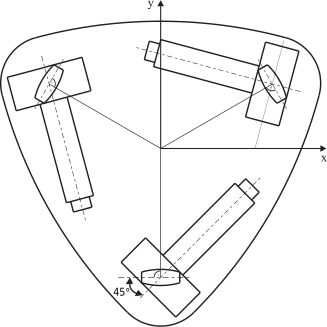
\includegraphics[width=1\textwidth]{figures/krikkit_drive_angles}
    \caption{\label{fig:omnidrive}Omni-drive schema of the Krikkit robot. Three $45^\circ$ Mecanum wheels have their small wheels arranged in a circle around the centre.
    \cite{mecanum2007}}
  \end{minipage}\hfill
  \begin{minipage}{0.45\textwidth}
   \centering
    \includegraphics[width=1\textwidth]{figures/Omniwheel_drive.png}
    \caption{\label{fig:mec-wheel}Mecanum wheel with motor and gearbox.}
  \end{minipage}
\end{figure}


The Krikkit robots served well for four years, much was learned.
Before RoboCup~2009 in Graz, a major mechanics overhaul was done.
In the meantime, all major electronic components also reached the end of their life cycle.
With the knowledge gained, lost and acquired again the successor of the Krikkit generation is in development now.
    

\subsection{In Development: Krikkit3G}

The next generation of robots is in development since mid-2010.
It will be a direct successor of the Krikkit generation, therefore the name \emph{Krikkit3G}.
The successful concepts are are adopted nearly unchanged:

\begin{itemize}
  \item omnidirectional drive with the three Mecanum Wheels
  \item the omni-vision system
  \item pneumatic kicking concept
  \item the use of a standard mini-ITX industrial PC
  \item modularity of all components
\end{itemize}

The new robot design focuses on the strict modularity of all components.
It has been shown that fast disassembling and replacing of critical components is crucial in the fast-paced tournament environment.
Especially the power train has been modularised, the wheel, gearing, motor and motor electronics can be swapped as a whole group.

Tests showed that the smoothness of the Mecanum wheels was insufficient due to manufacturing imprecision.
The resulting vibrations should be filtered out by an independent wheel suspension.

%  bumpers ?

For the kicking system, the pneumatic principle was kept.
But it is now much more versatile. 
It can switch between high and flat kicks at full power, and side-kicks are also possible now.
It features a new ball guidance system, which allows grabbing the ball for a short moment.
This becomes especially useful when decelerating.

Big changes were made in the electronics sector.
A new microcontroller core (An ARM Cortex~M3) is used on every component, replacing the different microcontroller architectures used before.
The smart battery system also got a major upgrade, featuring even smarter batteries.

In the mechanical design, space is now also provided for an improved odometry system, which will be developed based on this work.


\begin{figure}[b]
\begin{center}  
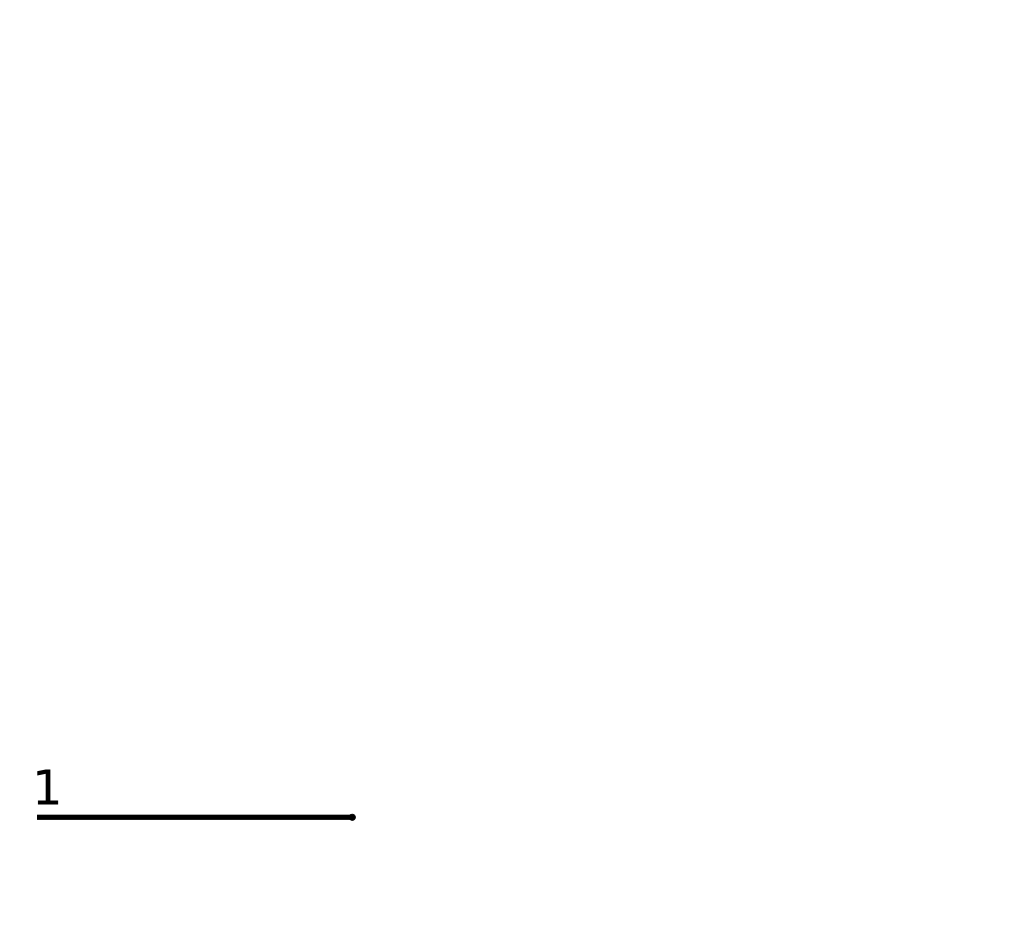
\includegraphics[width=0.5\columnwidth]{figures/Krikkit3G.jpg}
\caption{\label{fig:krikkit3g}
Rendering of the Krikkit3G robot (Without outer hull).
}   
\end{center}
\end{figure}


% 1p

\subsection{Odometry}

%  Definition
%  Verwendungsmoeglichkeit
%    Lokalisierung
%      higher framerate than cam
%      backup-system for cam
%    Motion control
%      anti-slip regulation

Odometry, better known as path measurement is important for every moving vehicle, especially robots which need to know where they currently are. 
The best known odometry measuring is used in cars as kilometre reading on the tachometer.

For autonomous mobile robots, odometry plays an even more important role.
Together with the vision system and the compass, it is a part in the sensor fusion for building the world model.
In the current Krikkit software, is is used for the following purposes:
At first, it acts as an initialisation vector for the vision system, when comparing two camera frames for calculating the offset between them.
The second important role comes from the high frequency odometry data is available.
Odometry data is provided with a frequency of 50\,Hz. 
This is much faster than the currently used vision system (15 - 25\,Hz). 
Therefore its values are added to the last known position in the world model for the time between two camera frames.
At last, it acts as a backup system for the mainly vision based localisation system in case of camera blackouts, e.g. blurred images due to the vibrations from a kick or a collision.

There are more possible use cases for odometry not implemented yet, e.g. anti-slip regulation for every single wheel.



\subsection{Motivation for this Work}
  
Current odometry systems of the Krikkit generation is based on the rotational speed of the wheels.
This has the major disadvantage of the accuracy bound to the slip of the wheels.
The problem is the non-uniform structure of the game field carpet, which has different slip factors in each direction.
Due to the different speeds and angles of the Mecanum wheels, this leads to deviations even when driving a straight line.
The errors accumulate over time, resulting in $90^\circ$~deviation on 10\,m straight distance driven.

Therefore, an wheel-independent odometry system has to be developed.
The goal of this work was:

\begin{itemize}
  \item Gathering requirements for a sensor
  \item Search for different types of sensors
  \item Implementation and validation of a prototype
\end{itemize}


\subsection{Requirements for a new type of Odometry Sensor on the Krikkit/3G platform}

The \MSL provides an ideal testbed for mobile robotics.
The main demands in robotics are miniaturisation, low cost and energy usage, and robustness to the environment.

The range of application in the \MSL demands the following design parameters:
\begin{itemize}
  \item must deliver linear and rotational accurate data in three degrees of freedom
  \item must work on green carpet, other surfaces are bonus.
  \item must not emit radiation or other disturbing effects irritating other robots or humans
  \item resistance against dust from the carpet abrasion
  \item shock resistant
\end{itemize}

The carpet is a particularly hairy concern, as its choice is up to the event organizer.
The only restriction in the \MSL rules and regulations~\cite{msl-rules} is: green.
Therefore, the game field surfaces differ in colour and surface roughness on every event.
Colours from bright green over dark teal to nearly grey have been seen over the past years.
The roughness is another chapter, it ranged from a very even felt with a roughness with a maximum of 2\,mm to an artificial grass like carpet with 15\,mm long hairs. 
Depending on the carpet the robot sinks in some millimetres, which also affects the clearance height.

The \MH requirements for a new odometry sensor are speeds of at least 5\,m/s at an operating frequency of at least 50\,Hz.
From the software side, it would be highly appreciated if the sensor would deliver data quality information.
Data quality information is crucial for the sensor fusion to recognize and de-prioritize erroneous data.
The \MH had bad memories about a malfunctioning compass ruining the world model.
At last, the \MH has very tight budgetary limitations, due to being a students-only team depending on external sponsors.
The sensors have to be cheap enough to be affordable for series for up to six robots.


On the Krikkit3G robots, the available space is limited to $50\times50\times110$\,mm for each of the three proposed sensor mount points.
The Krikkit3G robot, similar to the old Krikkit generation, has a clearance height of 20\,mm.
Due to the new independent wheel suspension, the operating range of the sensor must be greater than $\pm 5$\,mm to the reference plane.
Data must be output on the robot's CAN-Bus.
As power supply only two DC lines with 24\,V and 7\,V are available at reasonable currents.





\clearpage
\section{State of the Art}

\subsection{Odometry Measurement}

\subsubsection{Current Implementations used}

      wheel encoder
        probleme
      2. satz raeder
        probleme

\subsubsection{Possible Implementations}

      radar
1/4
      accelerometer
        2G spitzenvibration -> no
1/4
      Ultrasonic Doppler Velocimetry
1/4
      Microwave Doppler Velocimetry
1/4
      Laser interferometry
1/2
      Optical Spatial Frequency Filtration
1/4
        Daniel's approach
1/4
        laser speckle applications
        optical mice
1/2


\subsection{Decision for a Type of Sensor}
  entscheidung fuer einen Sensortyp
    - why/why not...
    - ...
    - ...


\section{Sensor Design}

block diagram
  ADNS + optic
  XC
  PC

\subsection{Optical System}
  requirements

micro-bench system

Sketch

\subsubsection{Optical Path calculations: Original Mouse Setup}

\subsubsection{Optical Path calculations: 2-Lens Setup}

\subsubsection{Optical Path calculations: Telecentric Setup}


\subsubsection{Sensor mounting \& Calibration}

Sketch with adjusting screws in all dimensions

calibration process
  laser

\subsubsection{Lens 2 \& Aperture Mounting}

manufacturing drawing

\subsubsection{Illumination}

  Why here?
  types of LEDs and Lasers used
 
  Illumination PCB

  circuit

  PCB print


\subsection{Electrical Design}

\subsubsection{The ADNS 6010}

specs

workflow diagram (from datasheet)

ADNS-testplatine
  requirements

  circuit diagram

  PCB drawing

\subsubsection{The XC164CM Microcontroller}

Specs etc

XC-164 eval board 
  Image from datasheet

Wiring of the Evaluation Board

  block diagram

  circuit

\subsection{Software}

\subsubsection{uC - Software}

  XC-Code
    requirements
    firmware catch

    image streaming

    motion data streaming
      + reference sensor

\subsubsection{PyQT GUI}

\subsubsection{Octave Analysis Scripts}

\section{Experimental Setup}

- requirements

\subsection{Mechanical Design of the Testbed}

block diagram

\subsection{Motor \& Disk}

\subsection{Reference Speed Sensor}
      Picture of sensor from Datasheet
      electrical setup used

\subsection{Microcontroller \& Host PC}      

\section{Experimental results}

\subsection{Illumination tests}

\begin{itemize}
  \item Laser
  \item Studio Spotlight
  \item ultra-bright white LEDs
  \item IR-LEDs
\end{itemize}

\subsection{Non-telecentric tests}

\subsection{Telecentric tests}

\subsubsection{Carpet 1}

\subsubsection{Carpet 2}

\subsubsection{Carpet 3}

\subsubsection{Game Field Lines}

\subsection{Interpretation}

  plots
  ergebnisse

\section{Conclusions \& Outlook}

  evaluation of a combination of IR-LED illumination and Laser illumination

  newer sensor ADNS-90xx

  mechanical limitations
    size constraints
    dirt cleaning...
  electrical requirements
    new architecture: ARM
    also include illumination control in uC
      use of the shuttered illumination for higher power 
      use of both LEDs and Lasers for white lines
  software algorithms: compute 3 dimension out of 2/4/6

ca 3-5p


summe gesamt 49 Seiten (ohne abstract, inhaltsv, bibl.)


%--------------------------------------------------------%
% Bibliography
%--------------------------------------------------------%
\addcontentsline{toc}{section}{Bibliography}
\label{Bibliography}
\bibliographystyle{plain}
\bibliography{literature}
%
\end{document}
